%Präambel
\documentclass[paper=a4,fontsize=11pt,headsepline,footsepline,parskip=half]{scrartcl}
\usepackage[utf8]{inputenc}
\usepackage[T1]{fontenc}
\usepackage{amsmath,amsfonts,amssymb}
\usepackage{ngerman,graphicx,textcomp,mathpazo,booktabs}
\usepackage[decimalsymbol=comma,per=frac]{siunitx}
\usepackage[textfont=sl,labelfont=bf]{caption}

%Seite einrichten
\areaset[2cm]		% Zusätzlicher Rand für die Bindung
        {17cm}{24cm}	% Textbreite und -Höhe

%Zeilenabstand
\linespread{1.2} %Standardwert

%Kopf- und Fußzeile
\usepackage{scrlayer-scrpage}
\setlength{\headheight}{23pt}
\lohead{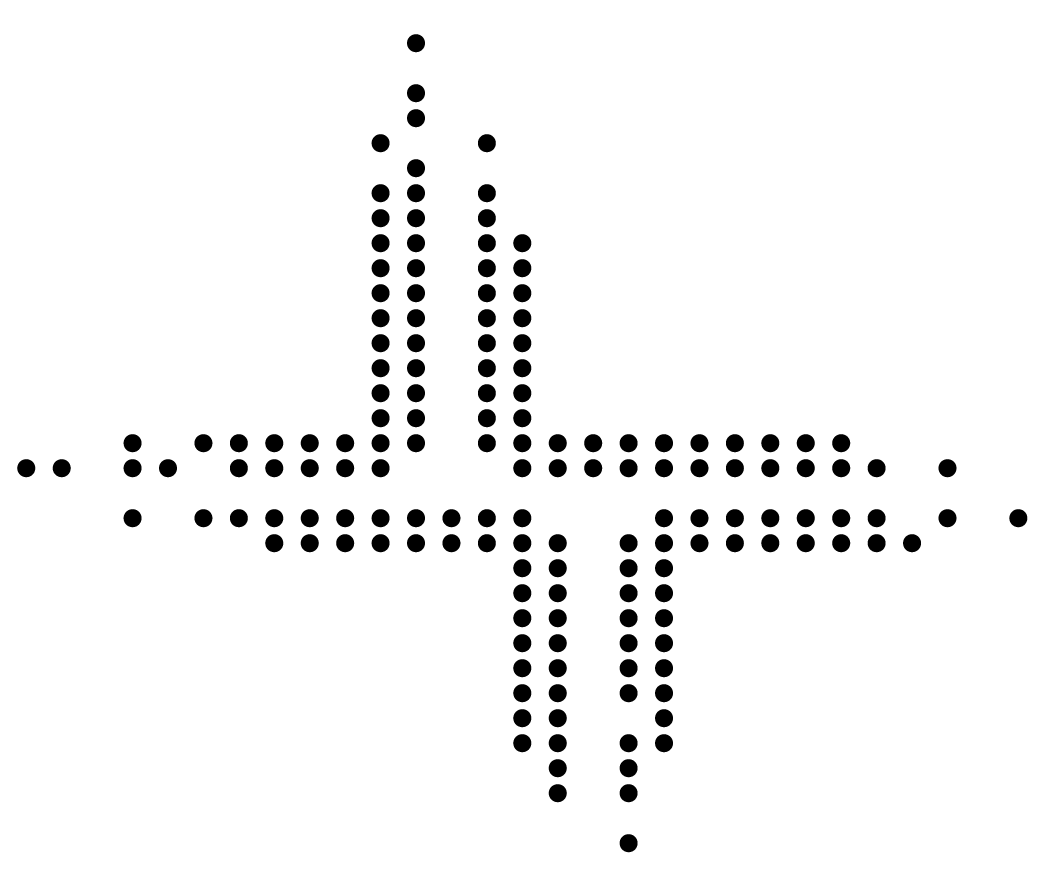
\includegraphics[width=0.7cm]{../logofbi} Hochschule Darmstadt}
\rohead{David Falk, Christian Lichtsinn}
\pagestyle{scrheadings}

%Programmierzeilen
\usepackage{listings}
%Optionen für listings
\lstset{
frame=single, %Rahmen
numbers=left %Zeilennummer
}

%sollte als letztes Paket geladen werden
\usepackage{hyperref}

\begin{document}

%Titelblatt
\begin{titlepage}

\begin{minipage}[c]{5cm}
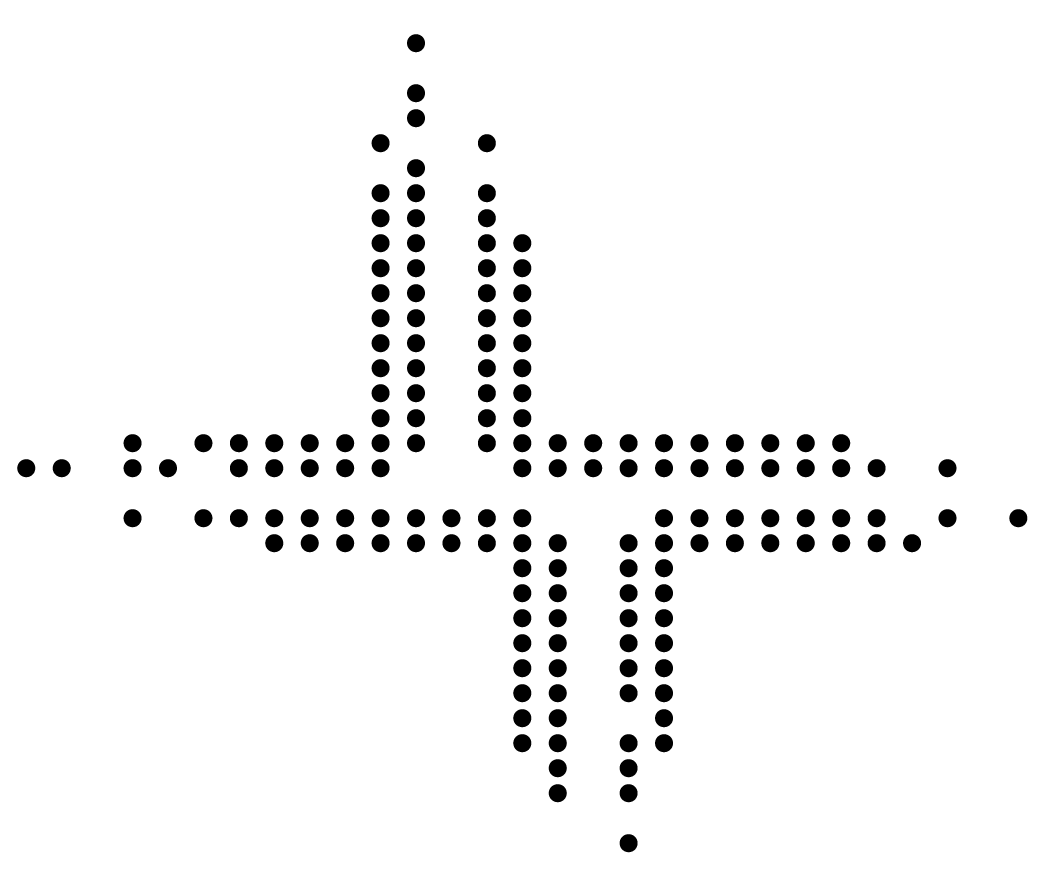
\includegraphics[width=5cm]{../logofbi}
\end{minipage}
\hfill
\begin{minipage}[c]{10cm}
\begin{flushright}
\Large Einführung in die Technik\\und Anwendung von\\
\LARGE \textbf{RFID}
\end{flushright}
\end{minipage}

\vspace*{1cm}

\begin{minipage}[c]{9cm}
\begin{flushleft}
\large David Falk (736532)\\Christian Lichtsinn (736787)\\Praktikum 3: 16.11.15: \textbf{Mo-56x}
\end{flushleft}
\end{minipage}
\hfill
\begin{minipage}[c]{7cm}
\begin{flushright}
\large Betreuer:\\Prof. Ralf S. Mayer\\F. Dotzauer
\end{flushright}
\end{minipage}

\vspace*{1cm}

%Workaround nötig wegen parskip Option.
\begingroup
  \setlength{\parskip}{0pt}% keinen Absatzabstand einfügen
  \setlength{\parindent}{0pt}% nicht einziehen
  \setlength{\parfillskip}{0pt plus 1fil}% Absatz darf komplett gefüllt sein
  \par\rule{\linewidth}{1.5pt}\par
\endgroup

\vspace*{\stretch{1}} %stretch zählt all stretch zusammen (hier 1+2=3) und verteilt den vspace entsprechend, hier 1/3

\centering
\Huge{\textbf{\textsl{RFID-LF-Reader\\ und Transponder}}}

\vspace*{\stretch{2}} %und hier 2/3 vspace vom Rest der Seite.

\end{titlepage}

%KAPITEL 1
\section{Fragen zu Atmel ATA2270-EK1}

\subsection{Wann darf das Reader-Board erst eingeschaltet werden?}

Erst wenn Reader-Board und die $125 kHz$-Antenne korrekt am Mainboard angebracht wurden, darf die Stromversorgung eingesteckt werden (und damit das Board eingeschaltet).

\subsection{Welche Spannung an der Spule ist zu erwarten?}

Es ist eine Spannung von $200 V$ zu erwarten.

\subsection{Wie ist die Induktivität der Antennenspule? Wie groß etwa wäre die dazugehörige Kapazität auf der Leser-Platine?}

Die Induktivität der Antennenspule wird mit $700 \mu H$ angegeben. Bei einer Resonanzfrequenz von $\omega_r = 125 kHz$ ergibt sich mit

\begin{align}
 \omega_r = \frac{1}{\sqrt{LC}} \Leftrightarrow C = \frac{1}{L \cdot \omega_r^2}
\end{align}

für die Kapazität $C = 91,429 nF$ auf der Leser-Platine.

\subsection{Was wäre zu beobachten, wenn eine andere Antennenspule mit unterschiedlicher Induktivität angeschlossen würde?}

Man müsste einen anderen Kondensator wählen, damit die Resonanzfrequenz $\omega_r = 125 kHz$ erreicht wird.

\subsection{Ist die mitgelieferte Antenne optimal?}

Die mitgelieferte Antenne ist eine Beispielantenne und nicht auf ein bestimmtes
Anwendungsszenario optimiert. %Diese Formulierung schwächt die Antwort ab. Sie verschleiert, dass wir nicht wissen, welche beiden
%optimalen Anwendungsszenarien wir kennen. Die vorherige Formulierung hat zumindest noch eine der beiden nennen können.

\subsection{Woraus besteht ein Tag (Transponder) im vorliegenden Kit?}

Ein Tag besteht aus einem integrierten Schaltkreis (intregrated circuit, IC), einem Kondensator und einer Antennenspule.

\subsection{Wie ist die Reihenfolge der gespeicherten und übertragenen Bits? Welcher Endian? Little oder Big?}

Die Blockreihenfolge ist von links nach rechts von 1 bis 32. Big Endian.

\subsection{Muss ein Tag initialisiert werden? Wann?}

Ein Tag ist zwar von Anfang an lesbar, aber muss natürlich für den Einsatz mit
sinnvollen Daten initialisiert werden.

\subsection{Welche Eigenschaften hat ein TK5551-Transponder?}

Ein TK5551-Transponder hat einen Konfigurationsblock und 7 Datenblöcke, jeder Datenblock speichert 32 Bits und damit insgesamt 224 Bits.

\subsection{Welche Eigenschaften hat ein ATA5577-Transponder?}

Ein ATA5577-Transponder hat einen Konfigurationsblock, 7 Datenblöcke à 32 Bits (zusammen 224 Bits) und 2 ID-Blöcken, sowie ein konfigurierbares
Analog-Frontend.

\subsection{Welche Besonderheiten hat ein ATA5570-Transponder?}

Je nachdem, ob die Impedanz hoch oder niedrig ist (was man mit dem Jumper J2
einstellen kann), werden die Daten korrekt oder invers versendet. Beschreibbar
ist der Tag nur bei niedriger Impedanz, also mit J2.

%KAPITEL 2
\section{Fragen zu SamSys-UHF-Reader}

\subsection{Wie ist das Lesegerät MP9320 in Betrieb zu nehmen, was ist zu beachten, wie wird die Antenne angeschlossen?}

Das Lesegerät verbindet man mit einem seriellem Kabel mit einem PC, damit man via einer Software mit dem Lesegerät kommunizieren kann. Das MP9320
darf dabei aber erst in Betrieb genommen werden, wenn entweder an den Antennenanschlüssen entsprechende UHF-RFID-Antennen angeschlossen sind oder
sich ein $50\ohm$-Abschlusswiderstand anstatt der Antenne befindet.

\subsection{Könnten mehrere UHF-Lesegeräte sich gegenseitig beeinflussen?}

TODO (Ja? Nein?)

\subsection{Was bedeutet ISO 18000-6?}

ISO 18000-6 ist eine Norm für die Spezifikation der Luftschnittstelle im UHF-Bereich (Ultra High Frequency) von $860 MHz$ bis $960 MHz$.

\subsection{Wie können Tags mit der RF Command Suite und der RS232-Schnittstelle gelesen werden?}

TODO

%KAPITEL 3
\section{ATA2270-EK RFID-Reader Praktikumsaufgaben}

Der ATA2270-EK RFID-Reader besitzt 4 F-Tasten und einen drückbaren Joystick. Mit allen F-Tasten geht man im Menü einen Menüpunkt zurück,
mit dem Joystick geht man durch das Menü und bestätigt mit Druck auf dem Joystick.

Eingestellt wird der Tag in dem Menüpunkt \textbf{select tag/reader}. Ausgelesen und beschrieben werden können die Datenblöcke des Tags
in dem Menüpunkt \textbf{read/write menu}. Dabei muss man beachten, dass der Datenblock erst beschrieben ist, nachdem man ihn mit
Druck auf den Joystick einzeln bestätigt.

\subsection{TK5551 und ATA5570 Transponder am Reader-Board}

Damit der Reader den Transponder auslesen kann, muss er erstmal entsprechend eingestellt werden.

Wir konnten den TK5551 Transponder auslesen, ihn neu beschreiben und den Transponder einer andernen Gruppe auslesen mit den Daten, die
diese in die Blöcke geschrieben haben.

Den ATA5570 Transponder konnten wir ebenfalls erfolgreich auslesen und wie erwartet wurden mit dem Abstecken von Jumper J2 die Daten in den Blöcken invertiert.

\subsection{ATA2270-EK1 via RS232-Schnittstelle am PC}

Um eine sinnvolle Ausgabe in TeraTerm zu bekommen, sollte man erst \textbf{local echo} einstellen, um nicht blind tippen zu müssen,
sowie die gesendeten Befehle und empfangenen Antworten auf \textbf{CR+LF} (carriage return + line feed) einstellen, damit die Ausgabe der
Befehle nicht überschrieben wird.

\subsubsection{Softwareversionsabfrage}

Die Softwareversion kann man mit folgenden Befehl abfragen und erhält dann die entsprechende Antwort, sofern alles ordentlich eingerichtet ist:

\begin{lstlisting}[caption={Softwareversionsabfrage.}]
 CMREV
 OK 0019 SW v3.4 Dec 17 2009
\end{lstlisting}

\subsubsection{HF anschalten und Transponder-Typ einstellen}

Das Hochfrequenzfeld wird mit folgenden Befehl angeschaltet:

\begin{lstlisting}[caption={HF anschalten.}]
 CMRFC1111ON
\end{lstlisting}

Um den Transponder-Typ einzustellen, damit man den Transponder überhaupt auslesen kann, müsste man eigentlich

\begin{lstlisting}[caption={Transponder-Typ einstellen.}]
 CMSRT 5551
\end{lstlisting}

als Befehl eingeben, laut Dokumentation. Das hat aber nicht funktioniert und wir haben auch nicht herausgefunden, wie man das via TeraTerm
einstellt, deswegen haben wir das am Reader-Board selbst durchgeführt.

\subsubsection{Tag-Test}

Um zu testen, ob sich überhaupt ein Tag im HF-Feld befindet oder nicht, nutzt man folgenden Befehl und erhält als Antwort entweder \glqq 
No Tag\grqq{} oder \glqq Tag Present\grqq.

\begin{lstlisting}[caption={Vorhandensein des Tags im HF-Feld testen.}]
 CMKTIF
 OK 0007 No Tag
 OK 0011 Tag Present
\end{lstlisting}

\subsubsection{Tag auslesen}

Die beiden folgenden Befehle

\begin{lstlisting}[caption={Tag auslesen.}]
 RDRTS 32
 RDRSS 32
\end{lstlisting}

lesen die ersten 32 bit aus.

\subsubsection{Modulationsart ändern}

Mit \textbf{MAN} für \glqq Manchester\grqq{}, \textbf{BP1} für \glqq Bi-Phase1\grqq{} und \textbf{BP2} für \glqq Bi-Phase2\grqq{} kann
man die Modulationsart entsprechend ändern. Im folgenden findet man die Befehle und die Datenausgabe vom ersten Datenblock vom gleichen
Transponder:

\begin{lstlisting}[caption={Modulationsart ändern und Ausgabe anzeigen.}]
 RDSRM0000MAN
 RDRSS 32
 000EEEEE
 RDSRM0000BP1
 RDRSS 32
 FFFEFFFF
 RDSRM0000BP2
 RDRSS 32
 33300000
\end{lstlisting}

\subsection{ATA5577 und ATA5570 Transponder via RS232-Schnittstelle am PC}

TODO (was noch dazu?)

Liest man die Herstellerdaten am Reader-Board aus, bekommt man folgende Darstellung:

\begin{tabular}{ll}
 ACL: E0 & LotID: 55048\\
 MFC: 15 & Wafer\#: 09\\
 ICR: 01 & Die\#: 3843 
\end{tabular}

Via TeraTerm bekommt man mit folgenden Befehl diese Antwort für die Herstellerdaten:
 
\begin{lstlisting}[caption={Herstellerdaten auslesen.}]
 ANRMD
 E000006EF8000076
\end{lstlisting}

\section{Animal-ID: ISO 11748/11785}

Um die Daten aus Animal-ID-Chips auslesen zu können, gibt man folgenden Befehl ein und erhält zB. diese Antwort:

\begin{lstlisting}[caption={Animal-ID-Abfrage.}]
 ANRCA
 OK 0030 1 0 0276 098102187461 672F OK
\end{lstlisting}

Nur was bedeuten die Zahlen jetzt, die man erhalten hat? Animal-IDs werden nach ISO 11784 und 11785 spezifiziert. 11784 beschreibt dabei
die Code-Struktur. In dieser wird beschrieben, dass die Zahl \textbf{276} nach der ISO-Ländercodierung 3166 für Deutschland steht. Danach
folgt gewöhnlich eine 0 und dann eine dreistellige Zahl, die den Hersteller identifiziert, in diesem Falle Datamars (981). Die Zahlen danach
sind laufende Herstellungsnummern.

\section{SamSys-UHF-Reader}

Aufgrund von Software-Problemen konnten wir diese Testreihe nicht durchführen.

\end{document}
